\documentclass[12pt,addpoints]{repaso}
\grado{2}
\nivel{Secundaria}
\cicloescolar{2023-2024}
\materia{Matemáticas}
\unidad{3}
\title{Practica la Unidad}
\aprendizajes{
    \item Usa e interpreta las medidas de tendencia central (moda, media aritmética y mediana), y decide cuál de ellas conviene más en el análisis de los datos en cuestión.
    \item Resuelve problemas de proporcionalidad directa e inversa y de reparto proporcional.
    \item Verifica algebraicamente la equivalencia de expresiones de primer grado, formuladas a partir de sucesiones.    
    \item Resuelve problemas mediante la formulación y solución algebraica de ecuaciones lineales.  
}
\author{Melchor Pinto, J.C.}
\begin{document}
\INFO%
\section*   {Probabilidad y estadística}
% \subsection*{Mediana y moda}
\ejemplosboxed[{Contesta las siguientes preguntas:

            \begin{multicols}{2}
                \begin{parts}
                    \part Las calificaciones de un salón de secundaria son las siguientes: 80, 82, 85, 88, 90, 88, 91, 85, 95, 88, 88, 97, 100. ¿Cuál es la mediana de las calificaciones?
                    \fillin[88][2cm]

                    \begin{solutionbox}{2cm}
                        Ordenando los datos se obtiene:\\[-0.2em]
                        $\left\{80, 82, 85, 85, 88, 88, 88, 88, 90, 91, 95, 97, 100 \right\} $\\[-0.2em]
                        $\therefore$ Mediana es 88
                    \end{solutionbox}

                    \part Las edades de un grupo de personas son: 44, 41, 47, 48, 44, 39, 45, 49, 44 y 47 años. ¿Cuál es la mediana de las edades?
                    \fillin[44.5][2cm]

                    \begin{solutionbox}{2cm}
                        Ordenando los datos se obtiene: \\[-0.2em]
                        $\left\{39, 41, 44, 44, 44, 45, 47, 47, 48, 49 \right\} $ \\[-0.2em]
                        $\therefore$ Mediana es 44.5
                    \end{solutionbox}

                \end{parts}
            \end{multicols}
        }]
\begin{questions}
    \questionboxed[4]{Contesta las siguientes preguntas:

        \begin{multicols}{2}
            \begin{parts}
                \part Las calificaciones de un salón de secundaria son las siguientes: 5, 7, 6, 8, 7, 9, 10, 7, 8, 7, 9, 7. ¿Cuál es la mediana de las calificaciones?
                \fillin[7][2cm]

                \begin{solutionbox}{1.8cm}
                \end{solutionbox}

                \part Las edades de un grupo de personas son: 15, 17, 15, 18, 19, 14, 15, 13 y 17 años. ¿Cuál es la mediana de las edades?
                \fillin[15][2cm]

                \begin{solutionbox}{1.8cm}
                \end{solutionbox}

            \end{parts}
        \end{multicols}
    }
    % \subsection*{Promedio}

    \ejemplosboxed[{Contesta las siguientes preguntas:

                \begin{multicols}{2}
                    \begin{parts}
                        \part El número de goles en las últimas 3 temporadas de un delantero fueron: 22, 26 y 31, ¿cuál es el promedio de goles por temporada?
                        \fillin[26.33][2cm]

                        \begin{solutionbox}{2.5cm}
                            Para encontrar el promedio sumamos el total de goles en esas temporadas y luego dividimos esa suma por el número de temporadas. En este caso, el promedio es
                            $(22+26+31)/3=26.33$
                        \end{solutionbox}

                        \part En un grupo de 11 personas se registraron los siguientes pesos: 62, 64, 65, 59, 68, 72, 77, 71, 82, 69 y 76 kg. ¿Cuál es el promedio de los pesos?
                        \fillin[69.54][2cm]

                        \begin{solutionbox}{2.5cm}
                            Al sumar los pesos: 62 + 64 + 65 + 59 + 68 + 72 + 77 + 71 + 82 + 69 + 76 = 765 kg, y dividir por 11 personas, obtenemos un promedio de aproximadamente 69.55 kg.
                        \end{solutionbox}

                    \end{parts}
                \end{multicols}
            }]

    \questionboxed[4]{Contesta las siguientes preguntas:

        \begin{multicols}{2}
            \begin{parts}
                \part Las estaturas de un grupo de personas son: 171, 172, 168, 166, 164, 178 y 175 cm, ¿cuál es el promedio de la estatura de las personas?
                \fillin[170.57][2cm]

                \begin{solutionbox}{2cm}

                \end{solutionbox}

                \part En un grupo de 9 personas se registraron los siguientes pesos: 87, 60, 71, 74, 81, 80, 66, 74 y 79 kg. ¿Cuál es el promedio de los pesos?
                \fillin[74.66][2cm]

                \begin{solutionbox}{2cm}
                \end{solutionbox}

            \end{parts}
        \end{multicols}
    }

    % \subsection*{Interpretación de gráficas}
    \ejemplosboxed[{Los resultados de una encuesta se muestran en la siguiente gráfica de barras:

                \begin{multicols}{2}
                    \begin{parts}
                        \part  ¿Cuántas personas participaron en la encuesta? \fillin[95][2cm]
                        \part  ¿Cuál es la fruta menos preferida por las personas? \fillin[Naranja][2cm]
                        \part  ¿Cuál es la fruta preferida por las personas? \fillin[Manzana][2cm]

                        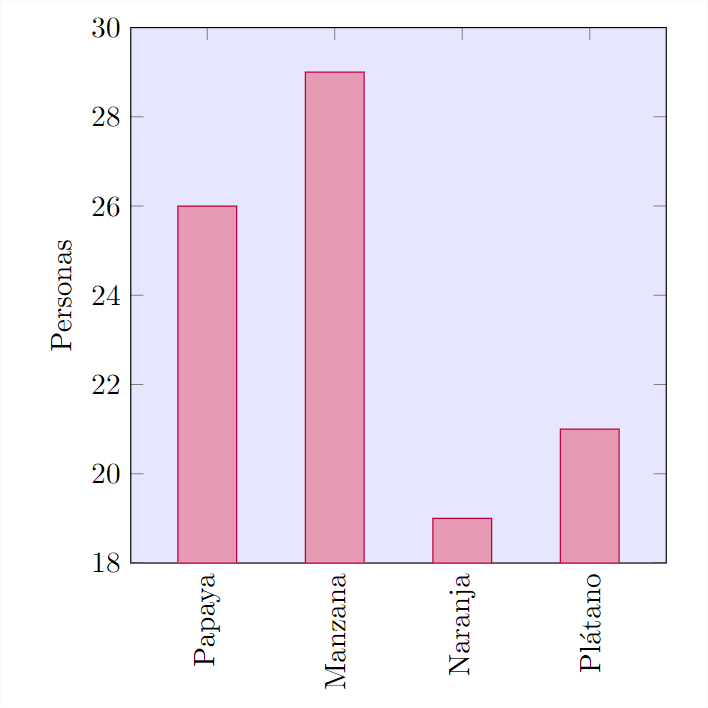
\includegraphics[width=.85\linewidth]{mexmat00001.png}
                    \end{parts}
                \end{multicols}
            }]

    \questionboxed[3]{Los resultados de una encuesta se muestran en la siguiente gráfica de barras:

        \begin{multicols}{2}
            \begin{parts}
                \part  ¿Cuántas personas participaron en la encuesta? \fillin[70][2cm]
                \part  ¿Cuál es la fruta menos preferida por las personas? \fillin[Papaya][2cm]
                \part  ¿Cuál es la fruta preferida por las personas? \fillin[Plátano][2cm]

                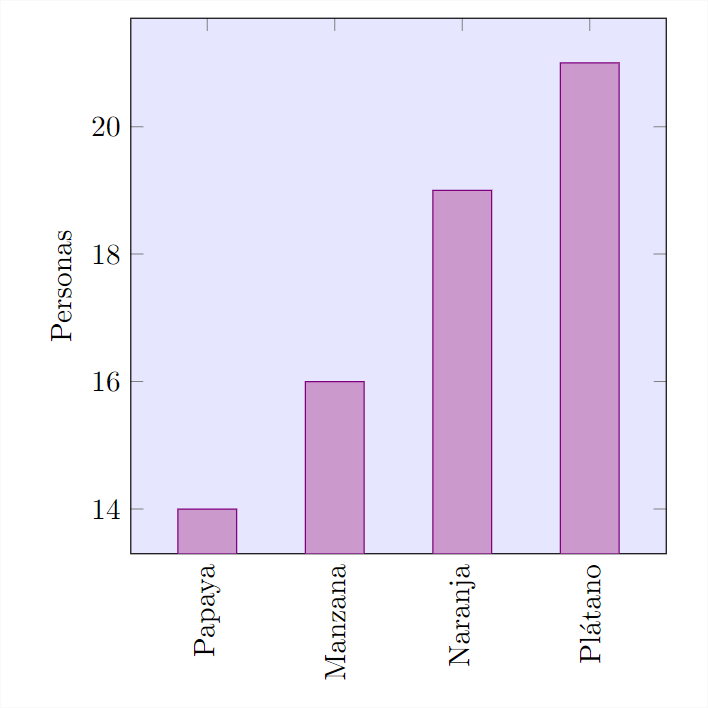
\includegraphics[width=.85\linewidth]{mexmat00001a.png}
            \end{parts}
        \end{multicols}
    }

    % \subsection*{Eventos mutuamente excluyentes}

    \questionboxed[3]{Resuelve los siguientes problemas:

        \begin{multicols}{3}

            \begin{parts}
                \part En una urna hay 10 pelotas azules, 5 verdes, 15 blancas y 20 negras. Calcula la probabilidad de sacar una pelota negra.

                \begin{solutionbox}{3cm}
                \end{solutionbox}

                \columnbreak%

                \part Si se lanzan tres monedas al aire, calcula la probabilidad de que caiga puro sol.

                \begin{solutionbox}{3cm}
                \end{solutionbox}

                \columnbreak%

                \part En una urna hay 8 pelotas moradas, 12 naranjas, 7 rojas, 11 azules y 7 blancas. Calcula la probabilidad de sacar una pelota negra.

                \begin{solutionbox}{3cm}
                \end{solutionbox}
            \end{parts}
        \end{multicols}
    }

    % \subsection*{Eventos dependientes e independientes}

    \questionboxed[3]{Resuelve los siguientes problemas:
        \begin{multicols}{2}

            \begin{parts}
                \part Se lanza una moneda al aire y al mismo tiempo un dado, ¿cuál es la probabilidad de que caiga águila en la moneda y el número 2 en el dado?
                \fillin[1/12][2cm]

                \begin{solutionbox}{2cm}
                \end{solutionbox}

                \part Al lanzar un dado tres veces consecutivas, ¿qué probabilidad hay de obtener en el primer dado un 2, en el segundo un 3 y en el tercero un número impar?
                \fillin[1/72][2cm]

                \begin{solutionbox}{2cm}
                \end{solutionbox}

            \end{parts}
        \end{multicols}
    }

    \section*   {Razones y proporciones}
    % \subsection*{Relaciones proporcionales}

    \ejemplosboxed[{Determina si las siguientes tablas de datos son o no una relación proporcional:

                \begin{multicols}{2}
                    \begin{parts}
                        \part
                        \begin{minipage}[t]{0.35\linewidth}
                            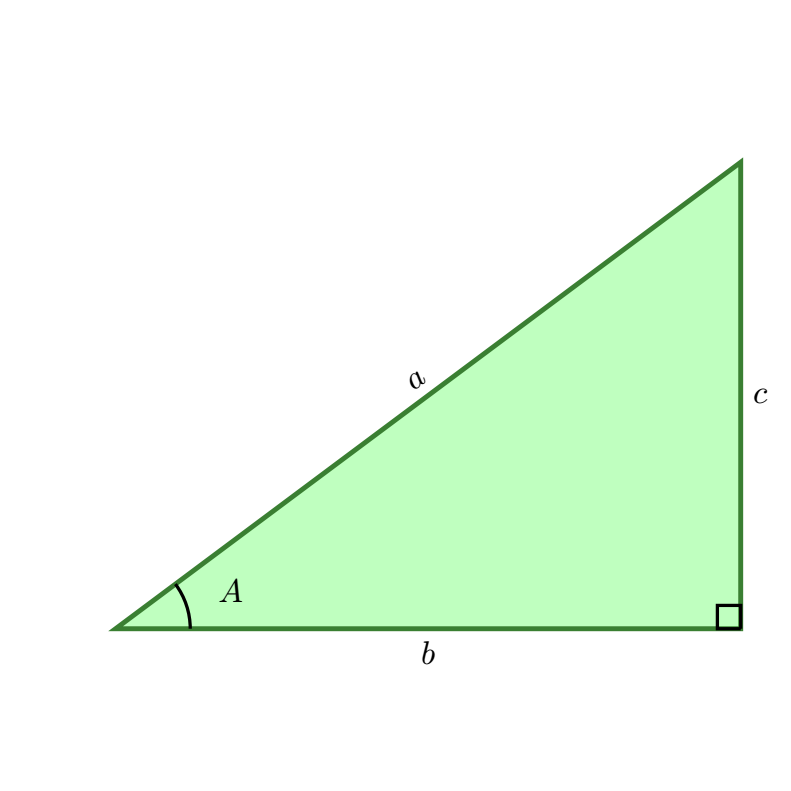
\includegraphics[width=\textwidth]{mex_0071.png}
                        \end{minipage}\hfill%
                        \begin{minipage}[b]{0.6\linewidth}
                            \begin{choices}
                                \choice Propocional
                                \CorrectChoice No proporcional
                            \end{choices}
                        \end{minipage}

                        \begin{solutionbox}{3cm}
                            $7\div 1=7$\\[-0.2em]
                            $9\div 2=4.5$\\[-0.2em]
                            $11\div 3=3.\overline{6}$\\[-0.2em]
                            $13\div 4=3.25$\\[-0.2em]
                            $15\div 5=3$\\[-0.2em]
                            $\therefore$ es una relación no proporcional.
                        \end{solutionbox}


                        % \part 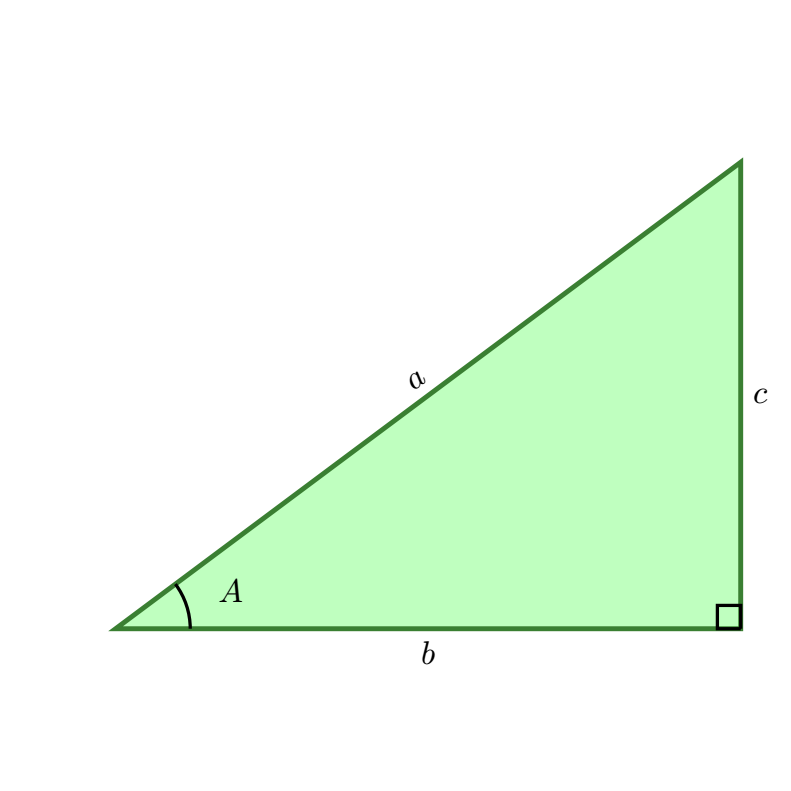
\includegraphics[width=.7\linewidth]{mex_0071.png}

                        % \begin{choices}
                        %     \choice Propocional
                        %     \choice No proporcional
                        % \end{choices}

                        \part
                        \begin{minipage}[t]{0.35\linewidth}
                            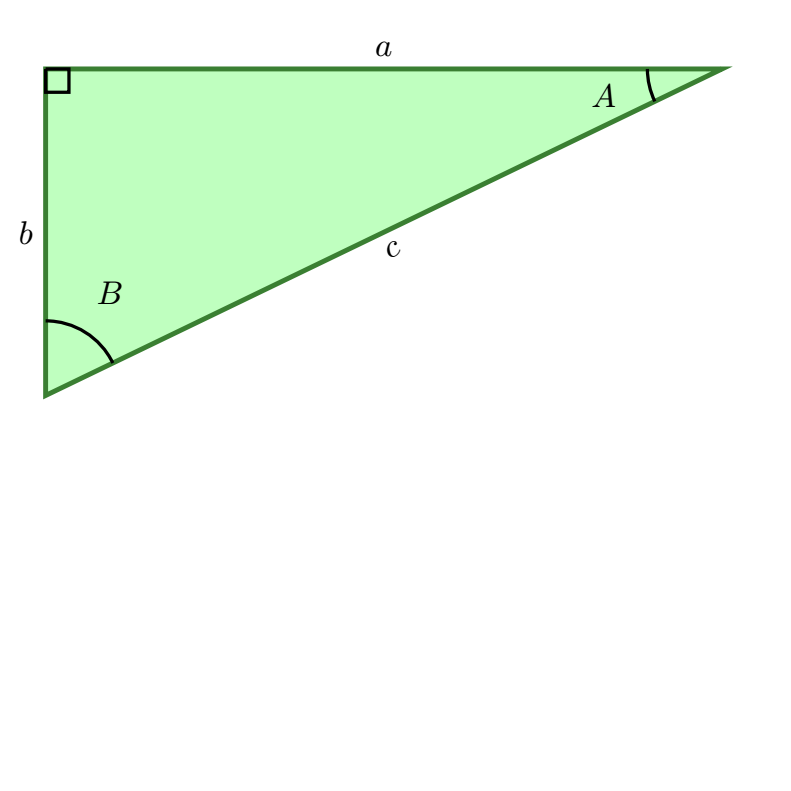
\includegraphics[width=\textwidth]{mex_0072.png}
                        \end{minipage}\hfill%
                        \begin{minipage}[b]{0.6\linewidth}
                            \begin{choices}
                                \CorrectChoice Propocional
                                \choice No proporcional
                            \end{choices}
                        \end{minipage}

                        \begin{solutionbox}{3cm}
                            $43.2\div 18=2.4$\\[-0.2em]
                            $33.6\div 14=2.4$\\[-0.2em]
                            $24\div 10=2.4$\\[-0.2em]
                            $14.4\div 6=2.4$\\[-0.2em]
                            $4.8\div 2=2.4$\\[-0.2em]
                            $\therefore$ es una relación proporcional.
                        \end{solutionbox}


                    \end{parts}
                \end{multicols}
            }]

    \questionboxed[6]{Determina si las siguientes tablas de datos son o no una relación proporcional:

        \begin{multicols}{2}
            \begin{parts}
                \part
                \begin{minipage}[t]{0.35\linewidth}
                    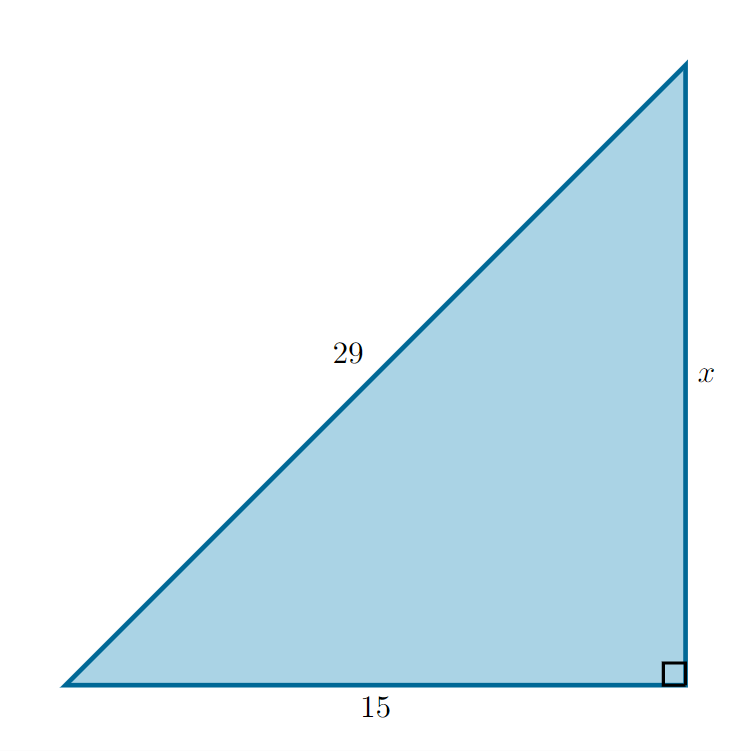
\includegraphics[width=\textwidth]{mex_0064.png}
                \end{minipage}%
                \begin{minipage}[b]{0.6\linewidth}
                    \begin{choices}
                        \choice Propocional
                        \CorrectChoice No proporcional
                    \end{choices}
                \end{minipage}

                \begin{solutionbox}{3cm}
                    $ 6\div 2=3$\\[-0.2em]
                    $12\div 4=3$\\[-0.2em]
                    $18\div 6=3$\\[-0.2em]
                    $24\div 8=3$\\[-0.2em]
                    $33\div 10=3.3$\\[-0.2em]
                    $\therefore$ es una relación no proporcional.
                \end{solutionbox}

                \part
                \begin{minipage}[t]{0.35\linewidth}
                    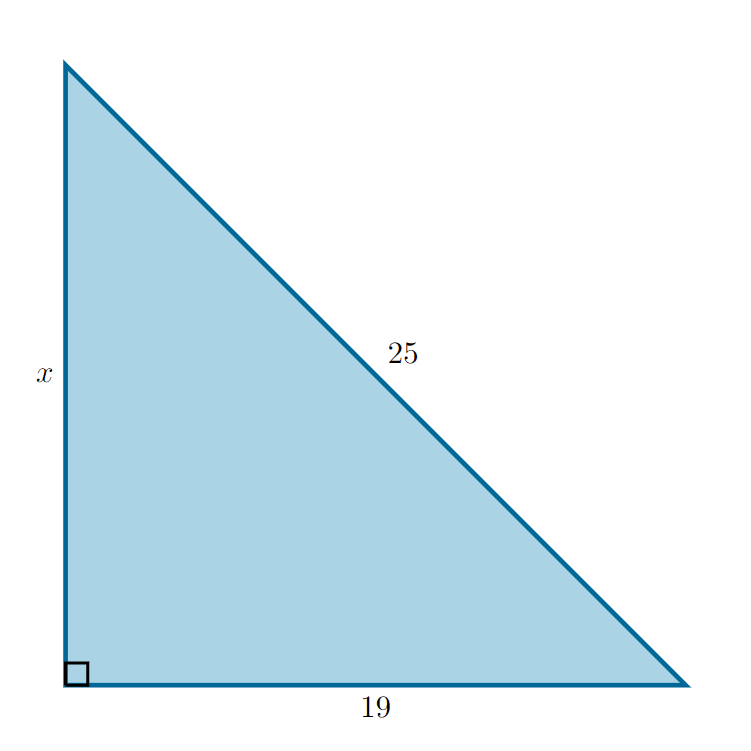
\includegraphics[width=\textwidth]{mex_0065.png}
                \end{minipage}%
                \begin{minipage}[b]{0.6\linewidth}
                    \begin{choices}
                        \CorrectChoice Propocional
                        \choice No proporcional
                    \end{choices}
                \end{minipage}

                \begin{solutionbox}{3cm}
                    $20\div  5=4$\\[-0.2em]
                    $36\div  9=4$\\[-0.2em]
                    $52\div 13=4$\\[-0.2em]
                    $68\div 17=4$\\[-0.2em]
                    $84\div 21=4$\\[-0.2em]
                    $\therefore$ es una relación proporcional.
                \end{solutionbox}

            \end{parts}
        \end{multicols}
    }

    % \subsection*{Constante de proporcionalidad}
    \ejemplosboxed[{Determina el valor de la constante de proporcionalidad para cada una de las siguientes tablas:

                \begin{multicols}{2}
                    \begin{parts}
                        \part
                        \begin{minipage}[t]{0.35\linewidth}
                            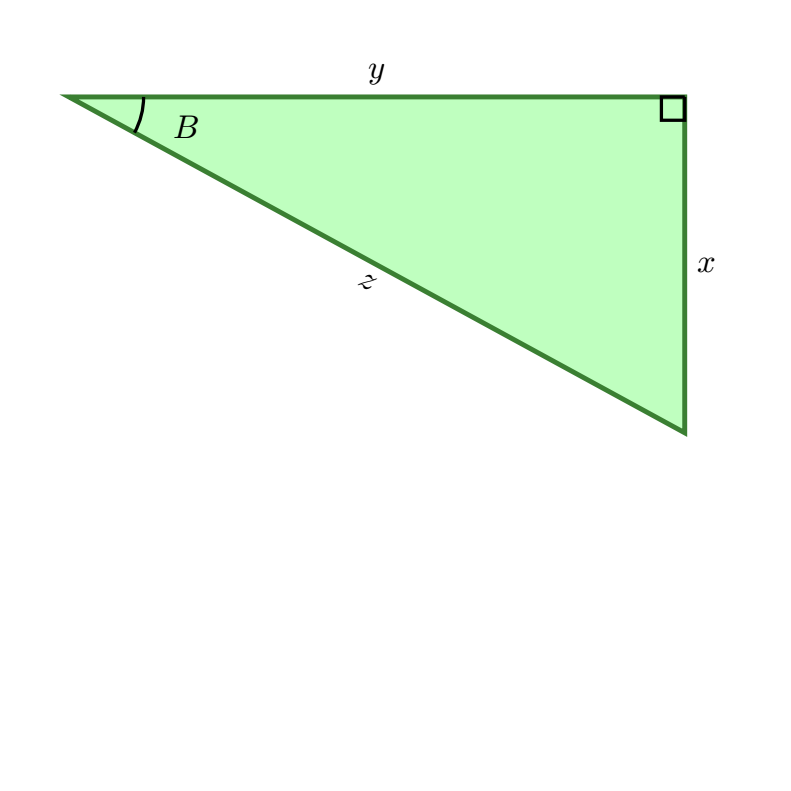
\includegraphics[width=\textwidth]{mex_0078.png}
                        \end{minipage}\hfill%
                        \begin{minipage}[b]{0.6\linewidth}
                            \begin{solutionbox}{2.8cm}\small%

                                \begin{multicols}{2}
                                    $ 2\div 1=2$\\[-0.2em]
                                    $ 4\div 2=2$\\[-0.2em]
                                    $ 6\div 3=2$\\[-0.2em]
                                    $ 8\div 4=2$\\[-0.2em]
                                    $10\div 5=2$

                                    \columnbreak% 

                                    $\therefore$ La constante de proporcionalidad es 2.
                                \end{multicols}
                            \end{solutionbox}
                        \end{minipage}


                        % \part 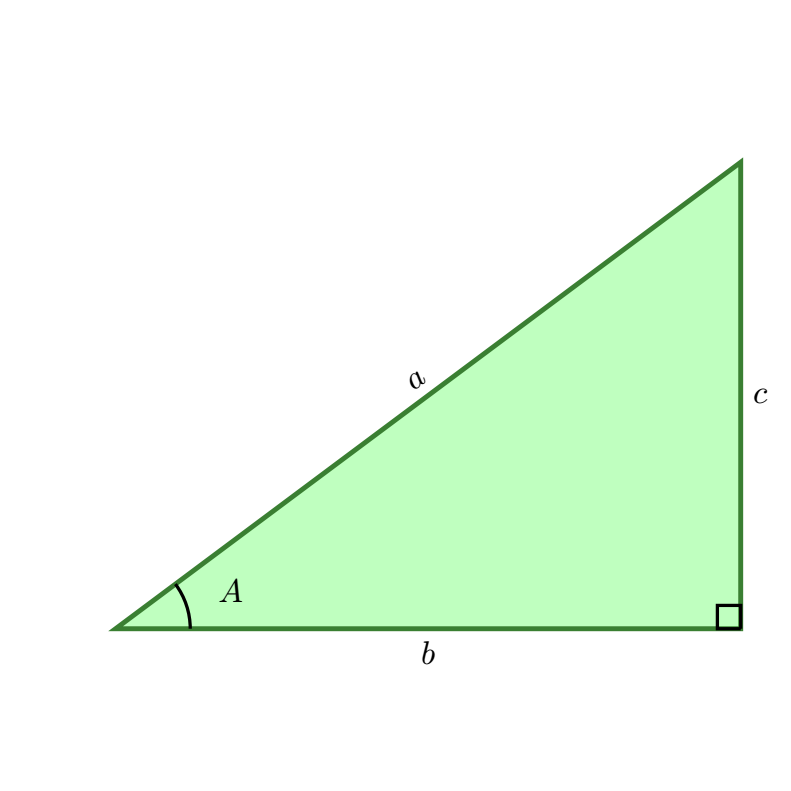
\includegraphics[width=.7\linewidth]{mex_0071.png}

                        % \begin{choices}
                        %     \choice Propocional
                        %     \choice No proporcional
                        % \end{choices}

                        \part
                        \begin{minipage}[t]{0.35\linewidth}
                            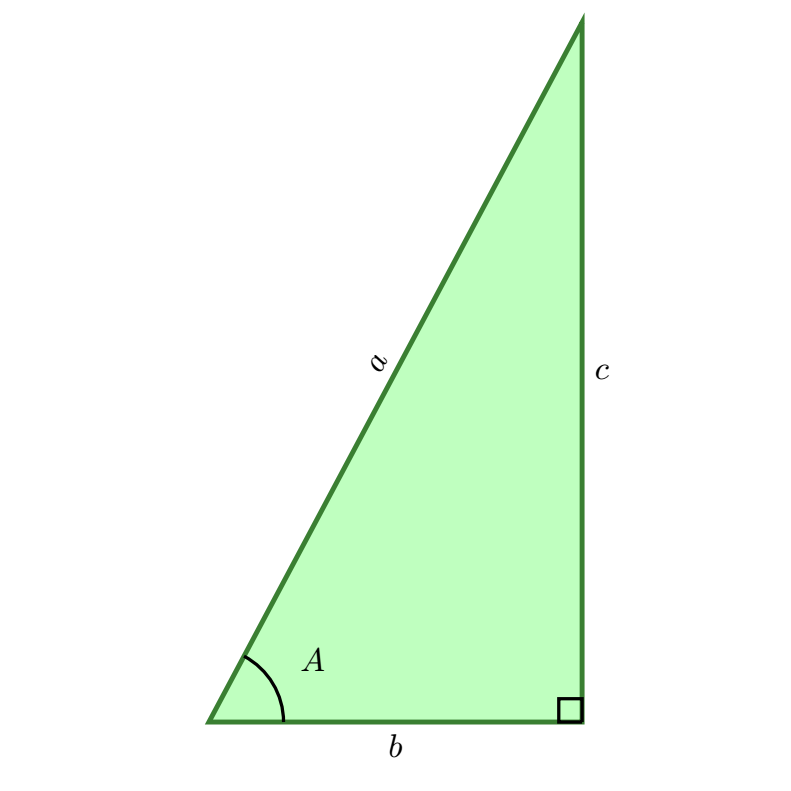
\includegraphics[width=\textwidth]{mex_0073.png}
                        \end{minipage}\hfill%
                        \begin{minipage}[b]{0.6\linewidth}
                            \begin{solutionbox}{3.5cm}\small%

                                \begin{multicols}{2}
                                    $\frac{16}{5}\div  4=\frac{4}{5}$\\[0.3em]
                                    $\frac{32}{5}\div  8=\frac{4}{5}$\\[0.3em]
                                    $\frac{48}{5}\div 12=\frac{4}{5}$\\[0.3em]
                                    $\frac{64}{5}\div 16=\frac{4}{5}$\\[0.3em]
                                    $16\div 20=\frac{4}{5}$

                                    \columnbreak%  

                                    $\therefore$ La constante de proporcionalidad es $\dfrac{4}{5}$.
                                \end{multicols}
                            \end{solutionbox}
                        \end{minipage}
                    \end{parts}
                \end{multicols}
            }]

    \questionboxed[6]{Determina si las siguientes tablas de datos son o no una relación proporcional:

        \begin{multicols}{2}
            \begin{parts}
                \part
                \begin{minipage}[t]{0.35\linewidth}
                    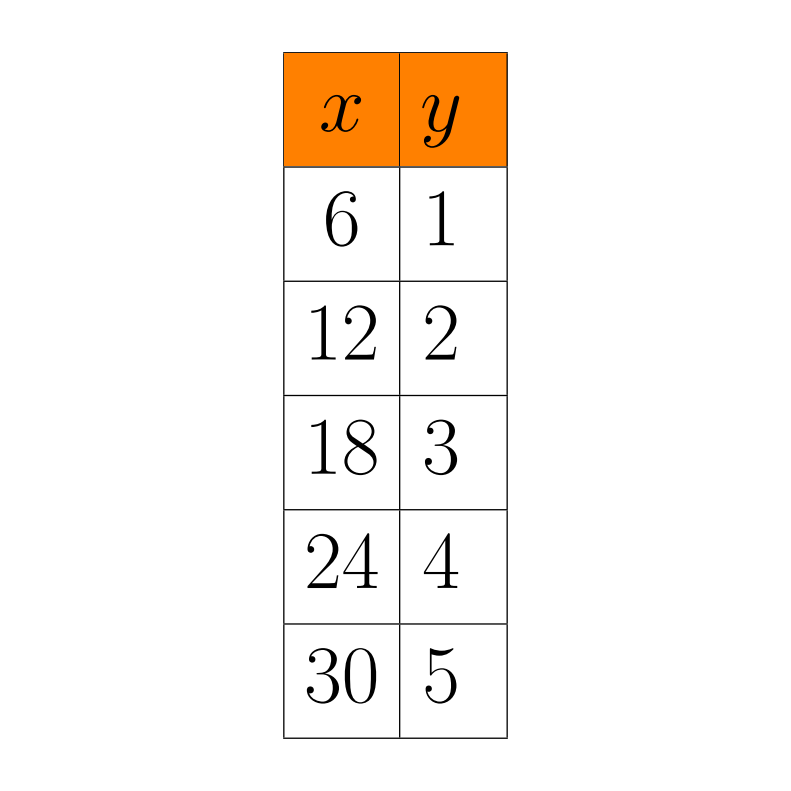
\includegraphics[width=\textwidth]{mex_0074.png}
                \end{minipage}%
                \begin{minipage}[b]{0.6\linewidth}
                    \begin{solutionbox}{3.5cm}\small%

                        \begin{multicols}{2}
                            $1\div  6=\frac{1}{6}$\\[0.3em]
                            $2\div 12=\frac{1}{6}$\\[0.3em]
                            $3\div 18=\frac{1}{6}$\\[0.3em]
                            $4\div 24=\frac{1}{6}$\\[0.3em]
                            $5\div 30=\frac{1}{6}$

                            \columnbreak% 

                            $\therefore$ La constante de proporcionalidad es $\dfrac{1}{6}$.                        \end{multicols}
                    \end{solutionbox}
                \end{minipage}

                \part
                \begin{minipage}[t]{0.35\linewidth}
                    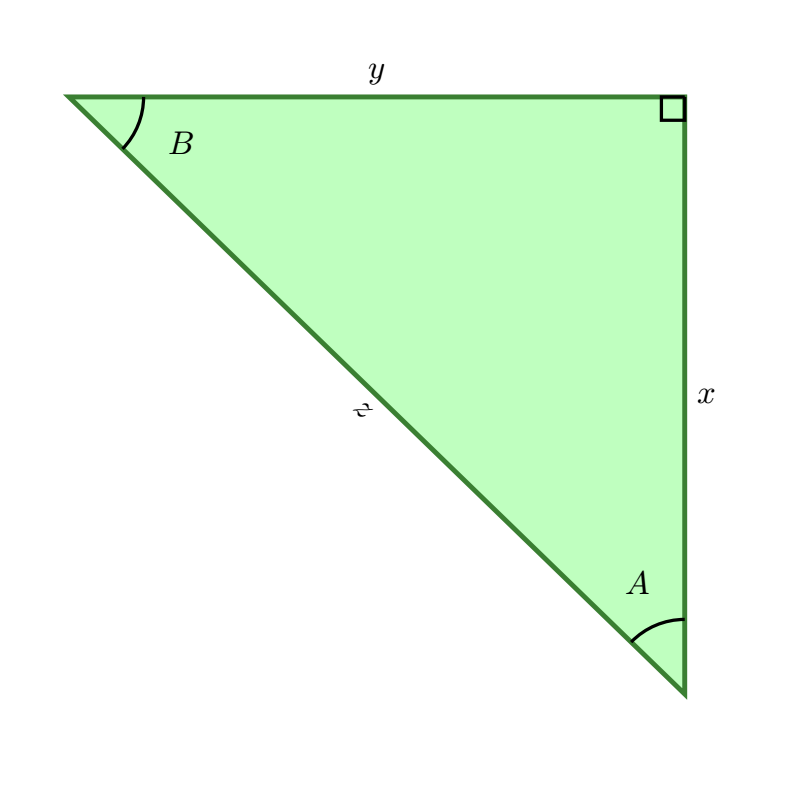
\includegraphics[width=\textwidth]{mex_0075.png}
                \end{minipage}%
                \begin{minipage}[b]{0.6\linewidth}
                    \begin{solutionbox}{3.5cm}\small%

                        \begin{multicols}{2}
                            $\frac{3}{4}\div  1=\frac{3}{4}$\\[0.3em]
                            $\frac{3}{2}\div  2=\frac{3}{4}$\\[0.3em]
                            $\frac{9}{4}\div 3=\frac{3}{4}$\\[0.3em]
                            $3\div 4=\frac{3}{4}$\\[0.3em]
                            $\frac{15}{4}\div 5=\frac{3}{4}$

                            \columnbreak%  

                            $\therefore$ La constante de proporcionalidad es $\dfrac{3}{4}$.
                        \end{multicols}
                    \end{solutionbox}
                \end{minipage}

                \part
                \begin{minipage}[t]{0.35\linewidth}
                    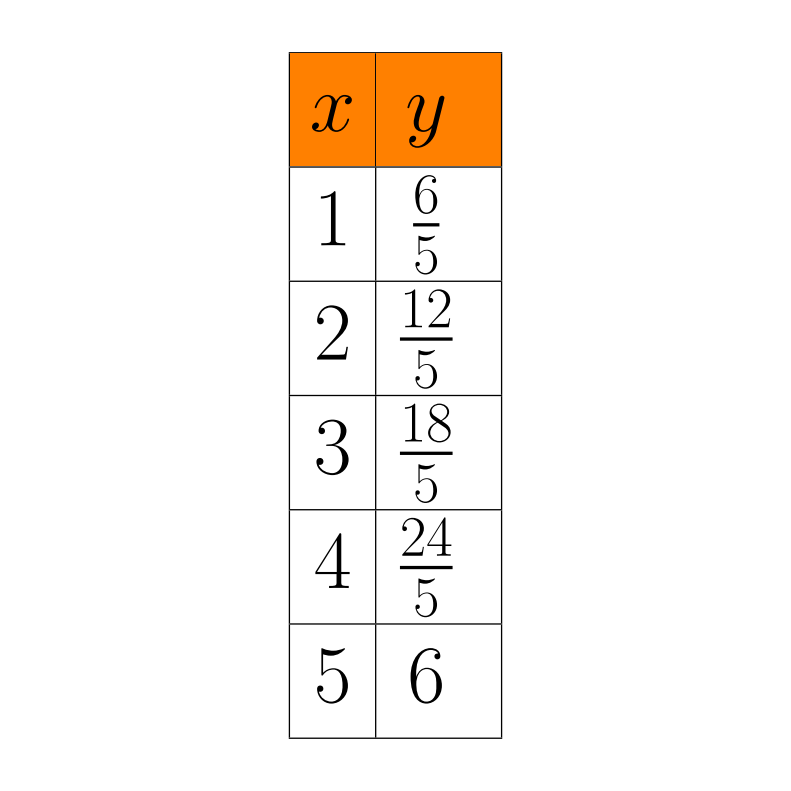
\includegraphics[width=\textwidth]{mex_0076.png}
                \end{minipage}%
                \begin{minipage}[b]{0.6\linewidth}
                    \begin{solutionbox}{3.5cm}\small%

                        \begin{multicols}{2}
                            $\frac{6}{5}\div  1=\frac{6}{5}$\\[0.3em]
                            $\frac{12}{5}\div 2=\frac{6}{5}$\\[0.3em]
                            $\frac{18}{5}\div 3=\frac{6}{5}$\\[0.3em]
                            $\frac{24}{5}\div 4=\frac{6}{5}$\\[0.3em]
                            $6\div 5=\frac{6}{5}$

                            \columnbreak%  

                            $\therefore$ La constante de proporcionalidad es $\dfrac{6}{5}$.
                        \end{multicols}
                    \end{solutionbox}
                \end{minipage}

                \part
                \begin{minipage}[t]{0.35\linewidth}
                    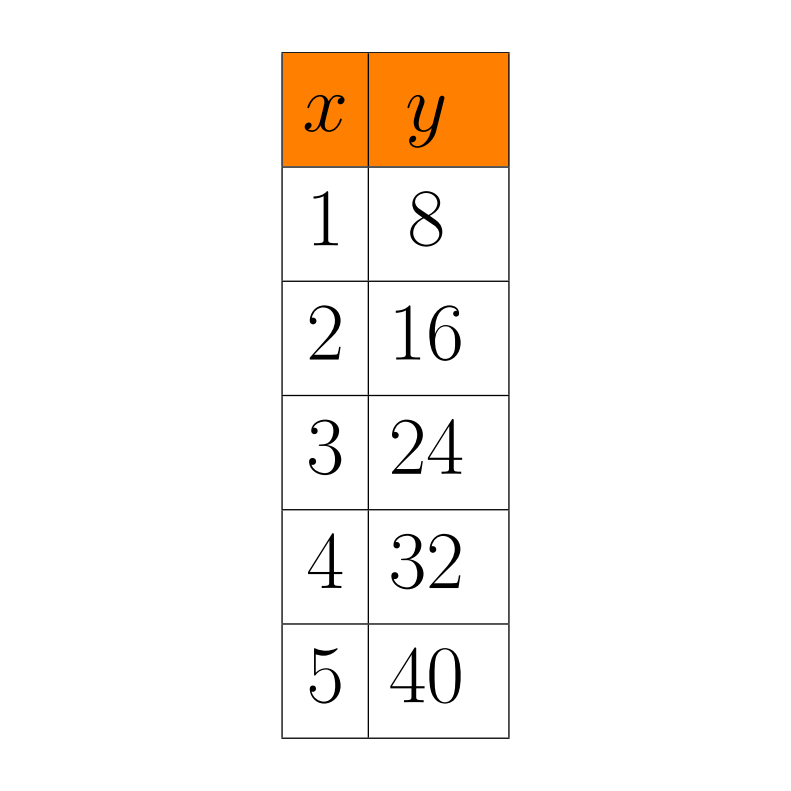
\includegraphics[width=\textwidth]{mex_0077.png}
                \end{minipage}%
                \begin{minipage}[b]{0.6\linewidth}
                    \begin{solutionbox}{2.8cm}\small%

                        \begin{multicols}{2}
                            $ 8 \div 1=8$\\[-0.2em]
                            $ 16\div 2=8$\\[-0.2em]
                            $ 24\div 3=8$\\[-0.2em]
                            $ 32\div 4=8$\\[-0.2em]
                            $ 40\div 5=8$

                            \columnbreak% 

                            $\therefore$ La constante de proporcionalidad es 8.
                        \end{multicols}
                    \end{solutionbox}
                \end{minipage}
            \end{parts}
        \end{multicols}
    }
    % \subsection*{Regla de correspondencia (ecuación)}
    \ejemplosboxed[{Escribe la regla de correspondencia (ecuación) de las siguientes tablas:

                \begin{multicols}{2}
                    \begin{parts}
                        \part%
                        \begin{minipage}[t]{0.25\linewidth}
                            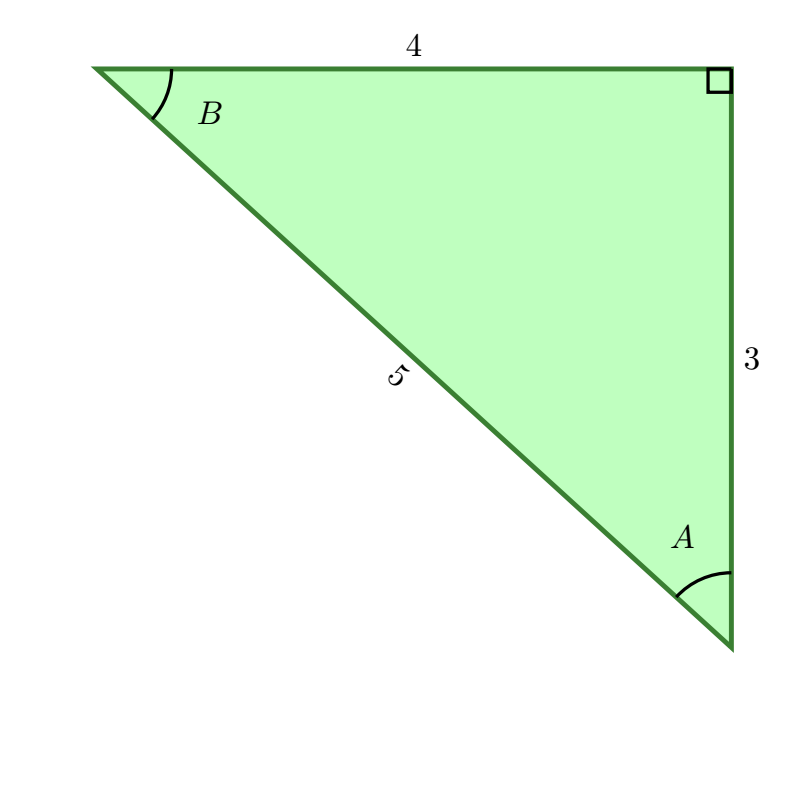
\includegraphics[width=2\linewidth]{mex_0082.png}
                        \end{minipage}\hfill%
                        \begin{minipage}[b]{0.6\linewidth}
                            \begin{solutionbox}{2cm}
                                La const. de prop. es $\frac{4}{5}$,

                                $\therefore$ la ecuación es $y=\frac{4}{5}x$.
                            \end{solutionbox}
                        \end{minipage}


                        % \part 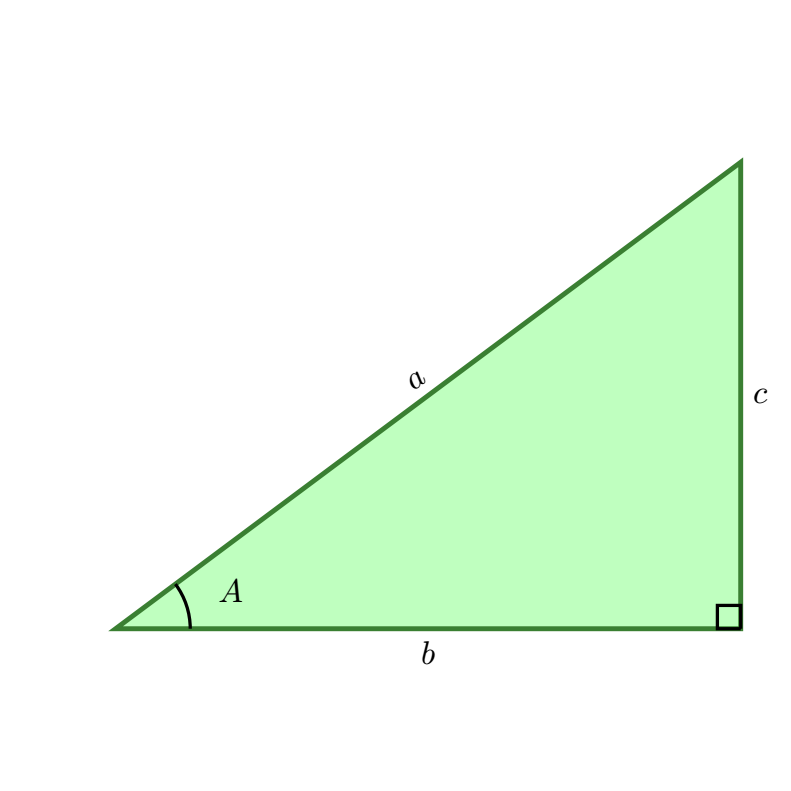
\includegraphics[width=.7\linewidth]{mex_0071.png}

                        % \begin{choices}
                        %     \choice Propocional
                        %     \choice No proporcional
                        % \end{choices}

                        \part%
                        \begin{minipage}[t]{0.25\linewidth}
                            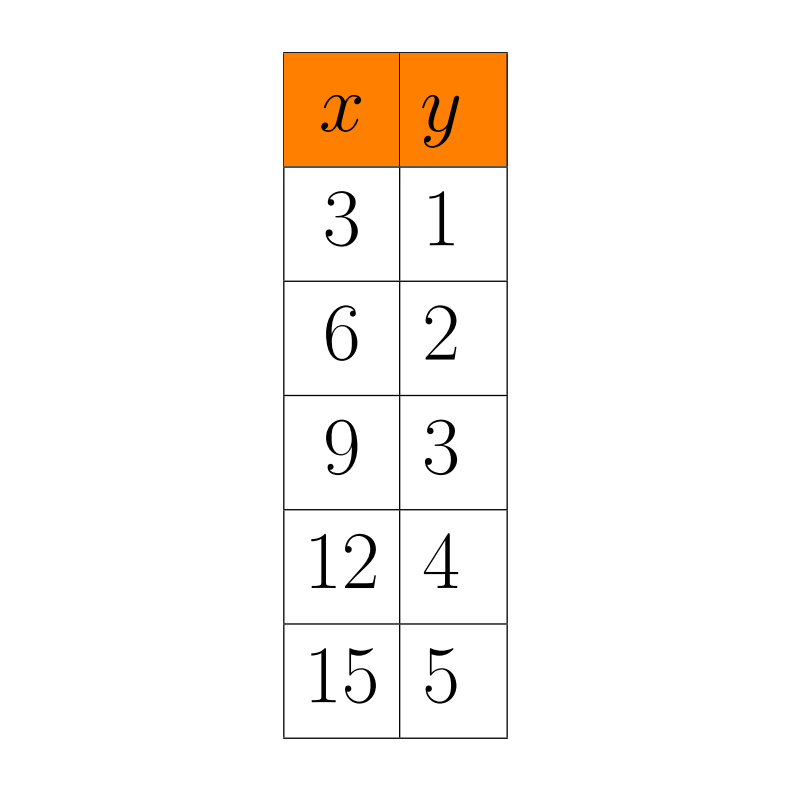
\includegraphics[width=2\linewidth]{mex_0083.png}
                        \end{minipage}\hfill%
                        \begin{minipage}[b]{0.6\linewidth}
                            \begin{solutionbox}{2cm}
                                La const. de prop. es $\frac{1}{3}$,

                                $\therefore$ la ecuación es $y=\frac{1}{3}x$.
                            \end{solutionbox}
                        \end{minipage}

                    \end{parts}
                \end{multicols}
            }]

    \questionboxed[6]{Escribe la regla de correspondencia (ecuación) de las siguientes tablas:

        \begin{multicols}{2}
            \begin{parts}
                % \part%
                % \begin{minipage}[t]{0.25\linewidth}
                %     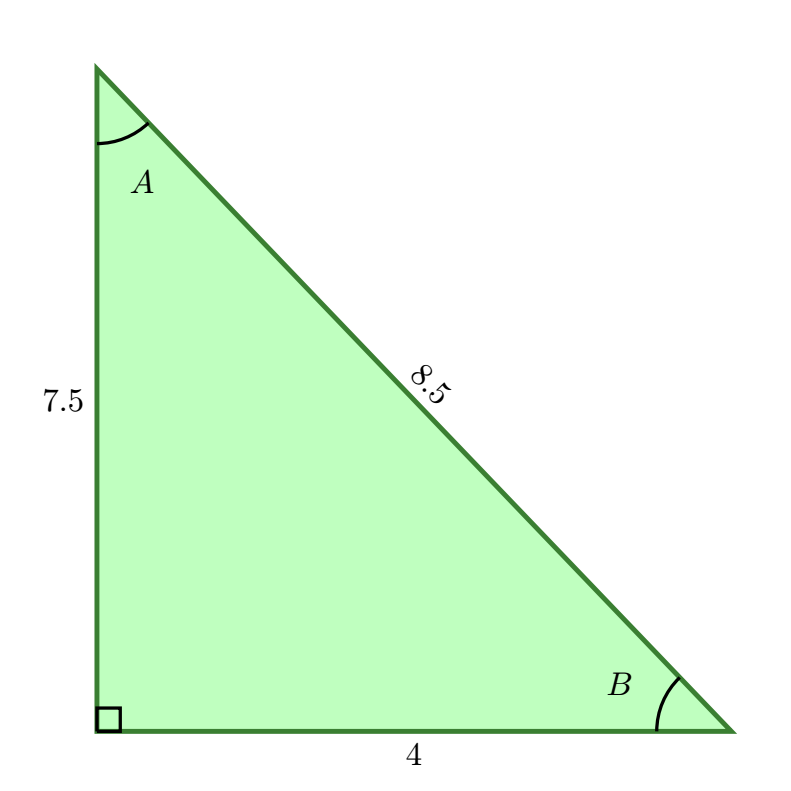
\includegraphics[width=2\linewidth]{mex_0084.png}
                % \end{minipage}\hfill%
                % \begin{minipage}[b]{0.6\linewidth}
                %     \begin{solutionbox}{2cm}
                %         La const. de prop. es $\frac{5}{1}$,

                %         $\therefore$ la ecuación es $y=5x$.
                %     \end{solutionbox}
                % \end{minipage}

                % \part%
                % \begin{minipage}[t]{0.25\linewidth}
                %     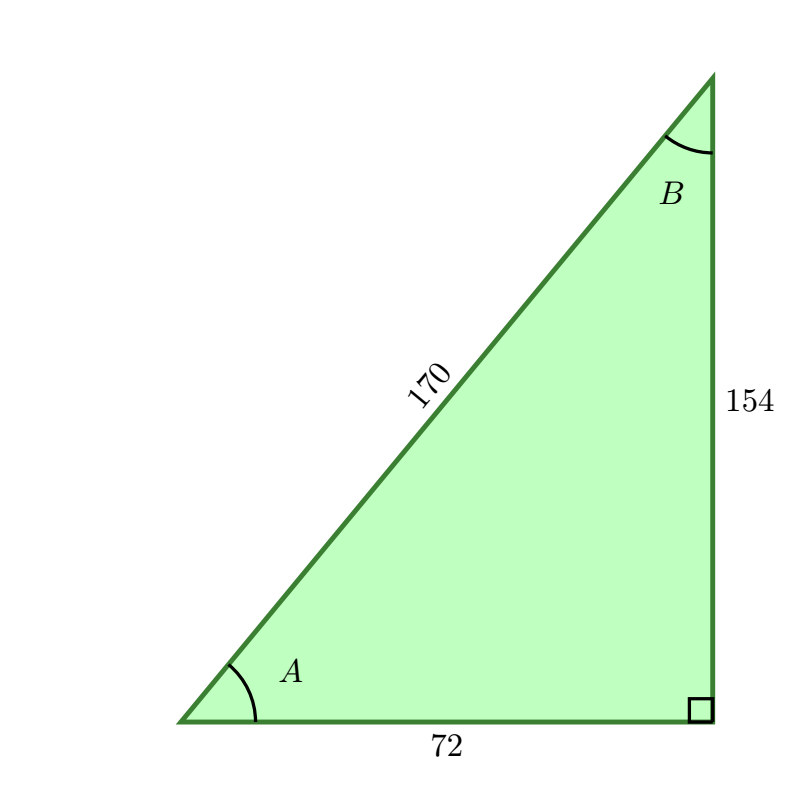
\includegraphics[width=2\linewidth]{mex_0085.png}
                % \end{minipage}\hfill%
                % \begin{minipage}[b]{0.6\linewidth}
                %     \begin{solutionbox}{2cm}
                %         La const. de prop. es $\frac{3}{1}$,

                %         $\therefore$ la ecuación es $y=3x$.
                %     \end{solutionbox}
                % \end{minipage}

                \part%
                \begin{minipage}[t]{0.25\linewidth}
                    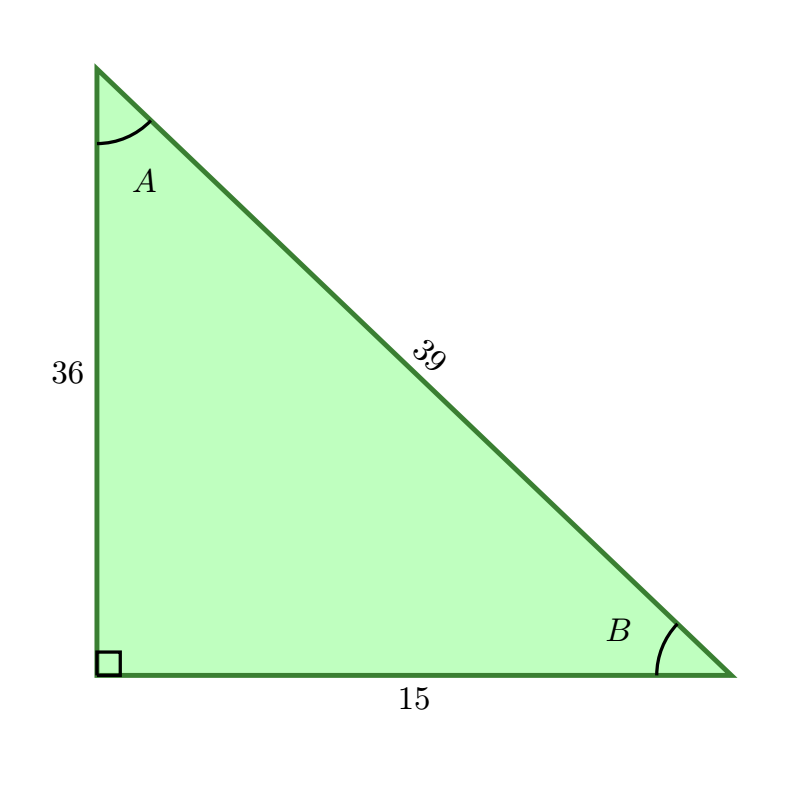
\includegraphics[width=2\linewidth]{mex_0086.png}
                \end{minipage}\hfill%
                \begin{minipage}[b]{0.6\linewidth}

                    \begin{solutionbox}{2cm}
                        La const. de prop. es $\frac{18}{15}=\frac{6}{5}$,

                        $\therefore$ la ecuación es $y=\frac{6}{5}x$.
                    \end{solutionbox}
                \end{minipage}

                \part%
                \begin{minipage}[t]{0.25\linewidth}
                    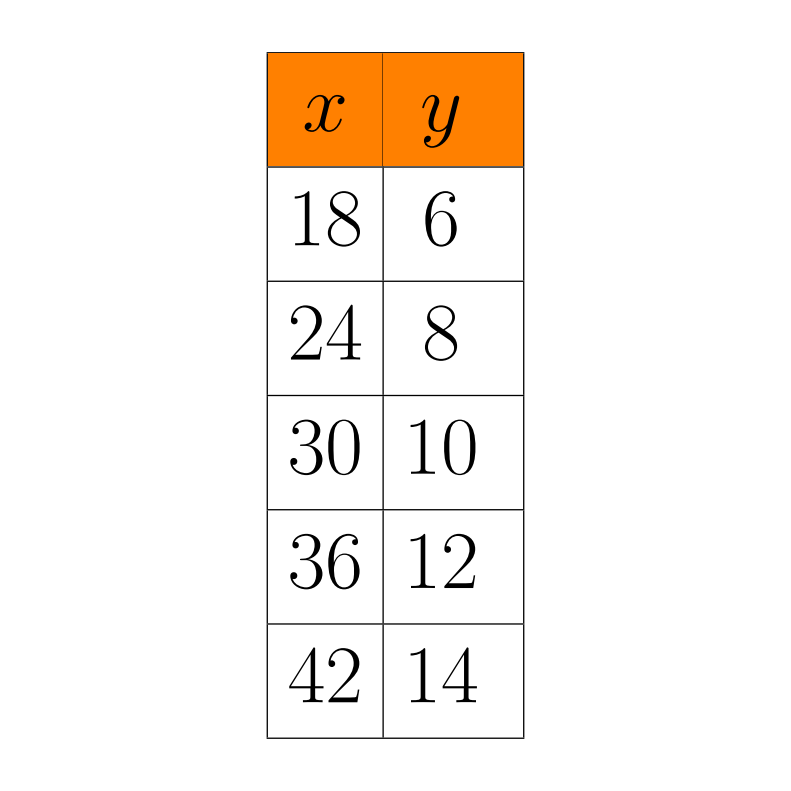
\includegraphics[width=2\linewidth]{mex_0087.png}
                \end{minipage}\hfill%
                \begin{minipage}[b]{0.6\linewidth}

                    \begin{solutionbox}{2cm}
                        La const. de prop. es $\frac{6}{18}=\frac{1}{3}$,

                        $\therefore$ la ecuación es $y=\frac{1}{3}x$.
                    \end{solutionbox}
                \end{minipage}

            \end{parts}
        \end{multicols}
    }

    % \subsection*{Proporción directa e inversa}
    \ejemplosboxed[{Resuelve los siguientes problemas:

                \begin{multicols}{2}
                    \begin{parts}
                        \part Si 8 trabajadores construyen un muro en 15 horas, ¿cuánto tardarán 5 trabajadores en construir el mismo muro?
                        \fillin[24][0.5cm]

                        \begin{solutionbox}{2cm}
                        \end{solutionbox}

                        \part Un grifo tiene un caudal de salida de 18 litros por minuto y tarda 14 horas en llenar un tanque. ¿Cuánto tardaría si el caudal fuera de 7 litros por minuto?
                        \fillin[36][0.5cm]

                        \begin{solutionbox}{2cm}
                        \end{solutionbox}
                    \end{parts}
                \end{multicols}
            }]

    \questionboxed[6]{Resuelve los siguientes problemas:
        \begin{multicols}{2}
            \begin{parts}
                \part Diez pintores tardan 16 días en pintar una casa, ¿cuánto tiempo tardarán en hacerlo 8 pintores?
                \fillin[20][0.5cm]

                \begin{solutionbox}{2cm}
                \end{solutionbox}

                \part 9 grifos abiertos durante 10 horas diarias han consumido una cantidad de agua por valor de 20 pesos. Calcula el precio del vertido de 15 grifos abiertos 12 horas durante los mismos días.
                \fillin[40][0.5cm]

                \begin{solutionbox}{2cm}
                \end{solutionbox}

                \part Una taladradora perfora 15 metros cada día trabajando 9 horas diarias. ¿Cuánto perforarán 2 taladradoras trabajando 6 horas diarias?
                \fillin[20][0.5cm]

                \begin{solutionbox}{2cm}
                \end{solutionbox}

                \part Si 3 grifos iguales tardan 5 horas en llenar un depósito de 10 m³, ¿en cuánto tiempo llenarían un depósito de 8 m³ 2 grifos como los anteriores?
                \fillin[6][0.5cm]

                \begin{solutionbox}{2cm}
                \end{solutionbox}
            \end{parts}
        \end{multicols}
    }
    % \subsection*{Proporciones compuestas}


    \section*   {Sucesiones aritméticas}
    % \subsection*{Completando la sucesión}
    \ejemplosboxed[{Escribe los términos faltantes de las siguientes sucesiones aritméticas:

                \begin{multicols}{3}
                    \begin{parts}
                        \part 28, 39, 50, \fillin[61][0.5cm], \fillin[72][0.5cm], \fillin[84][0.5cm], \dots
                        \part 56, 50, 44, \fillin[38][0.5cm], \fillin[32][0.5cm], \fillin[26][0.5cm], \dots
                        \part 33, 41, 49, \fillin[57][0.5cm], \fillin[65][0.5cm], \fillin[73][0.5cm], \dots
                    \end{parts}
                \end{multicols}%
            }]

    \questionboxed[6]{Escribe los términos faltantes de las siguientes sucesiones aritméticas:

        \begin{multicols}{3}
            \begin{parts}
                \part 21, 25, 29, \fillin[33][0.5cm], \fillin[37][0.5cm], \fillin[41][0.5cm], \dots
                % \part  4, 10, 16, \fillin[22][0.5cm], \fillin[28][0.5cm], \fillin[34][0.5cm], \dots
                \part 34, 31, 28, \fillin[25][0.5cm], \fillin[22][0.5cm], \fillin[19][0.5cm], \dots
                \part 92, 86, 80, \fillin[74][0.5cm], \fillin[68][0.5cm], \fillin[62][0.5cm], \dots
                % \part 51, 46, 41, \fillin[36][0.5cm], \fillin[31][0.5cm], \fillin[26][0.5cm], \dots
                % \part 250,225,200, \fillin[175][0.5cm], \fillin[150][0.5cm], \fillin[125][0.5cm], \dots
            \end{parts}
        \end{multicols}
    }

    % \subsection*{Diferencia de una sucesión}
    \ejemplosboxed[{Determina la diferencia de las siguientes sucesiones aritméticas:

                \begin{multicols}{2}
                    \begin{parts}
                        \part $-23,-15,-7,1,9,17,\ldots$ \fillin[$d=8$][0in]
                        \part $7,9,11,13,15,17,\ldots$ \fillin[$d=2$][0in]
                    \end{parts}
                \end{multicols}
            }]

    \questionboxed[4]{Determina la diferencia de las siguientes sucesiones aritméticas:

        \begin{multicols}{2}
            \begin{parts}
                \part $-15,-10,-5,0,5,\ldots$ \fillin[$d=5$][0in]
                \part $-8,-13,-18,-23,-28,-33,\ldots$ \fillin[$d=-5$][0in]
                \part $-19,-15,-11,-7,-3,1,\ldots$ \fillin[$d=4$][0in]
                \part $-4,-2,0,2,4,6,\ldots$ \fillin[$d=2$][0in]
            \end{parts}
        \end{multicols}
    }

    % \subsection*{Término enésimo}
    \ejemplosboxed[{Encuentra el \textit{n-ésimo} término de la siguientes sucesiones aritméticas:

                \begin{multicols}{2}
                    \begin{parts}
                        \part Calcula  el término número 44 de la siguiente sucesión aritmética: $a_n=-3n-15$

                        \begin{solutionbox}{1.5cm}
                            \[a_{44}=-3(44)-15=-132-15=-147\]
                        \end{solutionbox}

                        \part Calcula el término número 25 de la siguiente sucesión aritmética: $a_n=2n-6$

                        \begin{solutionbox}{1.5cm}
                            \[a_{25}=2(25)-6=50-6=44\]
                        \end{solutionbox}

                    \end{parts}
                \end{multicols}
            }]

    \questionboxed[6]{Encuentra el \textit{n-ésimo} término de la siguientes sucesiones aritméticas:
        \begin{multicols}{2}
            \begin{parts}
                \part Calcula el término número 45 de la siguiente sucesión aritmética: $a_n=-6n+10$

                \begin{solutionbox}{1.5cm}
                    \[a_{45}=-6(45)+10=-270+10=-260\]
                \end{solutionbox}

                \part Calcula el término número 37 de la siguiente sucesión aritmética: $a_n=4n+5$

                \begin{solutionbox}{1.5cm}
                    \[a_{37}=4(37)+5=148+5=153\]
                \end{solutionbox}

                \part Calcula el término número 55 de la siguiente sucesión aritmetica: $a_n=-2n+4$

                \begin{solutionbox}{1.5cm}
                    \[a_{55}=-2(55)+4=-110+4=-106\]
                \end{solutionbox}

                \part Calcula el término número 62 de la siguiente sucesión aritmética: $a_n=-5n+15$

                \begin{solutionbox}{1.5cm}
                    \[a_{62}=-5(62)+15=-310+15=-295\]
                \end{solutionbox}
            \end{parts}
        \end{multicols}
    }

    % \subsection*{Término general}
    \ejemplosboxed[{Determina el término general de las siguientes sucesiones aritméticas:
                \begin{multicols}{2}
                    \begin{parts}
                        \part $40,35,30,25,20,\ldots$ \fillin[$5-5n$][1in]
                        \part $-2,-6,-10,-14,-18,\ldots$ \fillin[$-4n+2$][1in]
                    \end{parts}
                \end{multicols}
            }]

    \questionboxed[4]{Determina el término general de las siguientes sucesiones aritméticas:
        \begin{multicols}{2}
            \begin{parts}
                \part $3,9,15,21,27,\ldots$ \fillin[$6n-3$][1in]
                \part $-69,-72,-75,-78,-81,\ldots$ \fillin[$-3n-66$][1in]
                \part $-2,1,4,7,10,\ldots$ \fillin[$3n-5$][1in]
                \part $-57,-65,-73,-81,-89,\ldots$ \fillin[$-8n-49$][1in]
            \end{parts}
        \end{multicols}
    }
    % \subsection*{Término enésimo 2}

    \ejemplosboxed[{Encuentra el \textit{n-ésimo} término de la siguientes sucesiones aritméticas:
                \begin{multicols}{2}
                    \begin{parts}
                        \part Calcula el término número 28 de la siguiente sucesión aritmética: $-69,-72,-75,-78,-81,\ldots$
                        \begin{solutionbox}{1.5cm}
                            \[-3(28)-66=-84-66=-150\]
                        \end{solutionbox}

                        \part Calcula el término número 47 de la siguiente sucesión aritmética: $-5,0,5,10,15,\ldots$
                        \begin{solutionbox}{1.5cm}
                            \[5(47)-5=235-5=225\]
                        \end{solutionbox}
                    \end{parts}
                \end{multicols}
            }]

    \questionboxed[4]{Encuentra el \textit{n-ésimo} término de la siguientes sucesiones aritméticas:
        \begin{multicols}{2}
            \begin{parts}
                \part Calcula el término número 15 de la siguiente sucesión aritmetica: $11,18,25,32,39,\ldots$

                \begin{solutionbox}{1.5cm}
                    \[7(15)+4=105+4=109\]
                \end{solutionbox}

                \part Calcula el término número 22 de la siguiente sucesión aritmética: $7,2,-3,-8,-13,\ldots$

                \begin{solutionbox}{1.5cm}
                    \[-5(22)+12=-110+12=-98\]
                \end{solutionbox}
            \end{parts}
        \end{multicols}
    }

    \section*   {Ecuaciones lineales}
    % \subsection*{Lenguaje algebraico}
    \ejemplosboxed[{Escribe la expresión algebraica correcta para los siguientes enunciados:
                \begin{multicols}{2}
                    \begin{parts}
                        \part El cuadrado de la diferencia de dos números cualquiera.

                        \begin{solutionbox}{1.3cm}
                            $(x-y)^2$
                        \end{solutionbox}

                        \part El cubo de un número cualquiera aumentado en 10.

                        \begin{solutionbox}{1.3cm}
                            $x^3+10$
                        \end{solutionbox}
                    \end{parts}
                \end{multicols}
            }]

    \questionboxed[6]{Escribe la expresión algebraica correcta para los siguientes enunciados:
        \begin{multicols}{2}
            \begin{parts}
                % \part La cuarta parte de un número cualquiera.

                % \begin{solutionbox}{1.3cm}
                %     $\dfrac{x}{4}$ o $\dfrac{1}{4}x$
                % \end{solutionbox}
                % \part El producto de tres números cualquiera.                \\ \fillin[$xyz$][0.5in]

                \part El cuadrado de la suma de dos números cualquiera.

                \begin{solutionbox}{1.3cm}
                    $(x+y)^2$
                \end{solutionbox}

                % \part El recíproco de un número cualquiera.

                % \begin{solutionbox}{1.3cm}
                %     $\dfrac{1}{x}$
                % \end{solutionbox}

                % \part El triple de un número cualquiera.

                % \begin{solutionbox}{1.3cm}
                %     $3x$
                % \end{solutionbox}

                % \part El doble del cuadrado de un número cualquiera.

                % \begin{solutionbox}{1.3cm}
                %     $2x^2$
                % \end{solutionbox}

                \part La mitad del cubo de la suma de dos números cualquiera.

                \begin{solutionbox}{1.3cm}
                    $\frac{1}{2}(x+y)^3$
                \end{solutionbox}

                % \part Dos novenas partes de un número cualquiera.

                % \begin{solutionbox}{1.3cm}
                %     $\frac{2}{9}x$
                % \end{solutionbox}

            \end{parts}
        \end{multicols}
    }


    % \subsection*{Sustitución de valores}
    \ejemplosboxed[{Encuentra el valor numérico de Las siguientes expresiones:

                \begin{multicols}{2}
                    \begin{parts}
                        \part $\large \dfrac{m-p}{n}$ cuando $m=8$, $n=5$ y $p=-2$.

                        \begin{solutionbox}{1.6cm}\footnotesize%
                            $\dfrac{m-p}{n}=\dfrac{8-(-2)}{5}=\dfrac{8´2}{5}=\dfrac{10}{5}=$ \fillin[2][0cm]
                        \end{solutionbox}

                        \part $\large a^{2}-2ab+b^{2}$ cuando $a=-4$ y $b=-7$.

                        \begin{solutionbox}{1.6cm}\footnotesize%
                            $a^{2}-2ab+b^{2}=(-4)^{2}-2(-4)(-7)+(-7)^{2}=16-56+49=$ \fillin[9][0cm]
                        \end{solutionbox}
                    \end{parts}
                \end{multicols}
            }]

    \questionboxed[6]{Encuentra el valor numérico de Las siguientes expresiones:

        \begin{multicols}{2}
            \begin{parts}
                \part $\large \left( \dfrac{x-y}{a+b} \right)^{3}$ cuando $a=-2$, $b=7$, $x=-6$ y $y=4$.

                \begin{solutionbox}{1.6cm}\footnotesize%
                    $\left( \dfrac{x-y}{a+b} \right)^{3}=\left( \dfrac{-6-4}{-2+7} \right)^{3}=\left( \dfrac{-10}{5} \right)^{3}=\left( -2 \right)^{3}=$ \fillin[-8][0cm]
                \end{solutionbox}

                \part $\large 5m-2n+x$ cuando $m=-3$, $n=4$ y $x=5$.

                \begin{solutionbox}{1.6cm}\footnotesize%
                    $5m-2n+x=5(-3)-2(4)+5=-15-8+5=$ \fillin[-18][0cm]\end{solutionbox}
            \end{parts}
        \end{multicols}
    }
    % \subsection*{Ecuaciones de primer grado 1}
    \ejemplosboxed[{Resuelve las siguientes ecuaciones:

                \begin{multicols}{3}
                    \begin{parts}
                        \part $ -x-2=15 $

                        \begin{solutionbox}{3.5cm}\footnotesize%
                            \begin{align*}
                                -x-2 & = 15                \\
                                -x   & =15+2               \\
                                -x   & =17                 \\
                                x    & = \frac{17}{-1}=-17
                            \end{align*}
                        \end{solutionbox}

                        \part $ 11x-33=55 $

                        \begin{solutionbox}{3.5cm}\footnotesize%
                            \begin{align*}
                                11x-33 & = 55            \\
                                11x    & =55+33          \\
                                11x    & =88             \\
                                x      & = \frac{88}{11}
                            \end{align*}
                        \end{solutionbox}

                        \part $\large -5x+9=-8x+3$

                        \begin{solutionbox}{3.5cm}\footnotesize%
                            \begin{align*}
                                -5x+9   & =-8x+3 \\
                                -5x     & =-8x-6 \\
                                -5x +8x & =-6    \\
                                3x      & =-6    \\
                                x       & =-2
                            \end{align*}
                        \end{solutionbox}
                    \end{parts}
                \end{multicols}
            }]

    \questionboxed[6]{Resuelve las siguientes ecuaciones:

        \begin{multicols}{2}
            \begin{parts}
                \part $\large -3(2x-5)=-1$

                \begin{solutionbox}{3.2cm}\footnotesize%
                    \begin{align*}
                        -3(2x-5) & =-1                           \\
                        -6x+15   & =-1                           \\
                        -6x      & =-1-15                        \\
                        -6x      & =-16                          \\
                        x        & =\sfrac{-16}{-6}=\sfrac{8}{3}
                    \end{align*}
                \end{solutionbox}

                \part $\large -4(3x+5)=5(-2x-3)$

                \begin{solutionbox}{3.2cm}\footnotesize%
                    \begin{align*}
                        -4(3x+5) & =5(-2x-3)                     \\
                        -12x-20  & =-10x-15                      \\
                        -12x+10x & =-15+20                       \\
                        -2x      & =5                            \\
                        x        & =-\sfrac{5}{-2}=-\sfrac{5}{2}
                    \end{align*}
                \end{solutionbox}
            \end{parts}
        \end{multicols}
    }

    % \subsection*{Ecuaciones de primer grado 2}


    % \subsection*{Resolución de problemas}
    \questionboxed[2]{Resuelve los siguientes problemas de ecuaciones lineales
        \begin{parts}
            \part La suma de tres números consecutivos es 195. Halla estos números

            \begin{solutionbox}{1.5cm}
            \end{solutionbox}

            \part La suma de dos números es 215 y el mayor excede al menor en 31 unidades. ¿Cuáles son estos dos números?

            \begin{solutionbox}{1.5cm}
            \end{solutionbox}
        \end{parts}

    }


    \section*   {Sistemas de ecuaciones}
    % \subsection*{Método de eliminación}
    % \subsection*{Método de sustitución}
    % \subsection*{Método de igualación}
    % \subsection*{Sistema de ecuaciones 2x2 1}
    % \subsection*{Sistema de ecuaciones 2x2}

    \questionboxed[8]{Utilizando el m\'etodo de tu preferencia, encuentra el valor de $x$ y $y$ para
        cada uno de los siguientes sistemas de ecuaciones lineales:
        \begin{multicols}{2}
            \begin{parts}
                \part
                \begin{align*}\Large%
                    2x+y & =  -10 \\
                    x-3y & =  2
                \end{align*}

                \begin{solutionbox}{4cm}
                    $x=-4$, $y=-2$
                \end{solutionbox}

                \part
                \begin{align*}\Large%
                    \frac{3}{5}x+\frac{1}{4}y & =  2   \\[1em]
                    x-5y                      & =   25
                \end{align*}

                \begin{solutionbox}{3cm}
                    $x=5$, $y=-4$
                \end{solutionbox}
                % \vspace{4cm}
            \end{parts}
        \end{multicols}
    }

    \questionboxed[3]{Numera correctamente los pasos para resolver un sistema de dos ecuaciones con dos inc\'ognitas por los m'etodos a continuaci\'on:
        \begin{choices}
            \choice M\'etodo de sustitución:
            \begin{itemize}
                \item[\rule{1cm}{0.2mm}] Despejar una inc\'ognita en una de las ecuaciones.
                \item[\rule{1cm}{0.2mm}] Resolver la ecuaci\'on resultante.
                \item[\rule{1cm}{0.2mm}] Sustituir el valor obtenido en la ecuaci\'on en la que aparec\'ia la inc\'ognita despejada.
                \item[\rule{1cm}{0.2mm}] Sustituir la expresi\'on de esta inc\'ognita en la otra ecuaci\'on para obtener una ecuaci\'on con una sola inc\'ognita.
                \item[\rule{1cm}{0.2mm}] Sustituir los valores en las ecuaciones originales para comprobar que son la soluci\'on.
            \end{itemize}

            \choice M\'etodo de suma-resta:
            \begin{itemize}
                \item[\rule{1cm}{0.2mm}] Resolver la ecuaci\'on resultante.
                \item[\rule{1cm}{0.2mm}] Sumar o restar las ecuaciones para eliminar una de las inc\'ognitas.
                \item[\rule{1cm}{0.2mm}] Sustituir los valores en las ecuaciones originales para comprobar que son la soluci\'on.
                \item[\rule{1cm}{0.2mm}] Multiplicar una o ambas ecuaciones por los n\'umeros necesarios para realizar la eliminaci\'on bajo la suma o resta.
                \item[\rule{1cm}{0.2mm}] Sustituir el valor obtenido en una de las ecuaciones iniciales y resolverla.
            \end{itemize}


            \choice M\'etodo de igualaci\'on:
            \begin{itemize}
                \item[\rule{1cm}{0.2mm}] Resolver la ecuaci\'on resultante.
                \item[\rule{1cm}{0.2mm}] Despejar la misma inc\'ognita en ambas ecuaciones.
                \item[\rule{1cm}{0.2mm}] Sustituir los valores en las ecuaciones originales para comprobar que son la soluci\'on.
                \item[\rule{1cm}{0.2mm}] Igualar las expresiones para obtener una ecuaci\'on con una inc\'ognita
                \item[\rule{1cm}{0.2mm}] Sustituir el valor obtenido en cualquiera de las dos expresiones en las que aparec\'ia despejada la otra inc\'ognita.
            \end{itemize}
        \end{choices}
    }

    \questionboxed[4]{Resuelve el siguiente sistema de ecuaciones lineales con decimales:
        \begin{align*}\Large%
            -0.2x+0.4y= & 0.6 \\
            x+2y=       & -3
        \end{align*}

        \begin{solutionbox}{4cm}
            $x=-3$, $y=0$
        \end{solutionbox}
    }

\end{questions}
\end{document}